\chapter{Verification of Deep Learning}\label{chap:verificationchap}

Successful experience from industrial software engineering, which produced software that is currently applied in safety-critical applications, such as automotive and avionic applications, suggests that, to develop high-quality and low-cost software in a limited production time, a software development life cycle (SDLC) process is required. As illustrated in Figure~\ref{fig:oldVmodel} about a V-model for SDLC, verification is a key process throughout the development lifecycle.   This chapter will discuss a specific verification task, i.e., given a trained machine learning model and a robustness property, it is to determine whether the robustness property holds on the model. After the definition of robustness property in Section~\ref{sec:robusntessproperty}, we will present representative examples for two categories of verification algorithms in Section~\ref{chap:MILP} and Section~\ref{chap:reachabilityAnalysis}, respectively. 
%
\begin{figure}[!htbp]
    \centering
    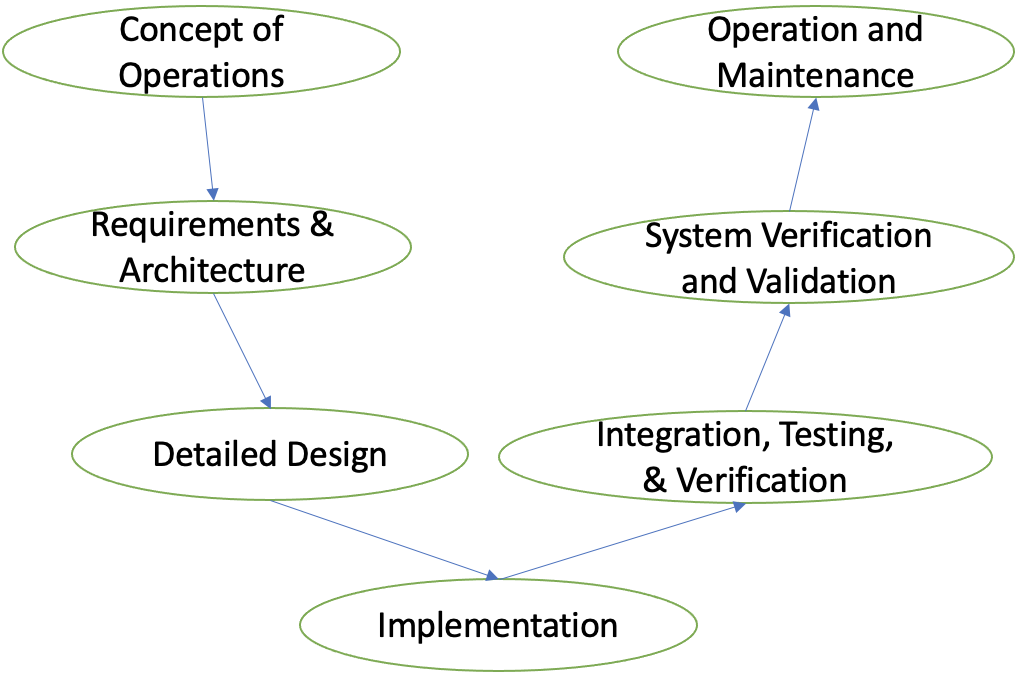
\includegraphics[width=0.6\textwidth]{images/robustnessVerification/oldVmodel.png}
    \caption{An illustrative V-model for software development}
    \label{fig:oldVmodel}
\end{figure}
%


%
Existing verification algorithms can be roughly categorised into exhaustive search \cite{HKWW2017}, constraint-solving based methods~%
%such as
\cite{katz2017reluplex}, abstract interpretation based methods~%
%such as
\cite{gehr2018ai,10.1007/978-3-030-32304-2_15},  global optimisation \cite{ruan2018global,RWSHKK2018}, game-based methods~\cite{wicker2018feature,wu2018game}, and symbolic interval analysis \cite{10.1007/978-3-030-32304-2_15,10.1145/3368089.3417918,10.1007/s00165-021-00548-1}. The readers are referred to \cite{HUANG2020100270} for a survey. 
%These methods ensure  the completeness and the soundness of the results. 
Moreover, in addition to the pixel perturbations measured with norm distances, we are also looking into real-world perturbations such as geometric and spatial perturbations \cite{GeoRobust2022}.  
%
This chapter presents a few typical verification algorithms. The first algorithm of this chapter (Section~\ref{chap:MILP}) reduces the verification to a constraint solving problem, which can then be solved with an off-the-shelf solver. The algorithm is white-box, and the reduction needs to consider the internal architecture of the neural networks. The complexity is NP-complete with respect to the combined number of hidden neurons and input features. 
%
On the other hand, the second algorithm (Section~\ref{chap:reachabilityAnalysis}), as some others  \cite{ruan2018global,RWSHKK2018,wicker2018feature,wu2018game,GeoRobust2022}, is black-box, i.e., they do not rely on the internal architecture of the neural networks. Theoretically, this brings a significant advantage that the computational complexity of the verification problem is NP-complete with respect to the number of input features. While the complexity class does not change, the number of hidden neurons can be an unlimited number of times more than that of input features, due to the current trend of deep learning on training deeper and larger networks. Also, black-box verification means that we can work with neural networks of any scale and structure. 

\section{Robustness Properties for Verification}\label{sec:robusntessproperty}

A (deep and feedforward) neural network, or neural network, can be defined as a tuple $\network=(\layers,
\layerConnections, \Phi)$, where $\layers=\{\layers_k~|~k\in\{1..K\}\}$ is a set of layers,
$\layerConnections\subseteq \layers\times \layers$ is a set of connections between layers and 
$\Phi=\{\phi_k~|~k\in\{2..K\}\}$ is a set of functions, one for each non-input layer.
%
%between layers
%$f_k:D_{L_{k-1}}\rightarrow D_{L_k}$ such that $D_{L_{k}}$ is the vector space of layer $k$. 
%
In a neural network, $\layers_1$ is the \emph{input} layer, $\layers_{K}$ is the \emph{output} layer,
and layers other than input and output layers are called \emph{hidden layers}.
Each layer $\layers_k$ consists of $s_k$ %nodes, which are also called
\emph{neurons} (or nodes).
The $l$-th node of layer $k$ is denoted by $n_{k,l}$.


Each node $n_{k,l}$ for $2 \leq k\leq K$ and  $1\leq l\leq s_k$ is associated with two variables $u_{k,l}$ and $v_{k,l}$, to record  its values before and after an activation function, respectively.
%
The Rectified Linear Unit (ReLU) \cite{relu} is one of the most popular 
%and effective 
activation functions for neural networks, according to which the \emph{activation 
value} of each node of hidden layers is defined as
%
\begin{equation}
    \label{eq:relu}
    v_{k,l}=ReLU(u_{k,l})=
    \begin{cases}
        u_{k,l} &\mbox{  if } u_{k,l}\geq 0 \\
            0 & \mbox{  otherwise}
    \end{cases}
\end{equation}
%\james{Definition (3) seems to put $u$ and $v$ as output and input - rather than as used in (2) as input and output respectively. Have I missed something here?}\xiaowei{it's ok}

%
Each input node $n_{1,l}$ for $1\leq l\leq s_1$ is associated with a
variable $v_{1,l}$ and each output node $n_{K,l}$ for $1\leq l\leq s_K$ is
associated with a variable $u_{K,l}$, because no activation function is
applied on them. Other popular activation functions beside ReLU include: Sigmoid, Tanh, and Softmax. 

% We use $u_{k,l}$ to denote
%the value of $n_{k,l}$. 
Except for the nodes at the input layer, every node is connected to nodes in the
preceding layer by pre-trained parameters such that for all $k$ and $l$ with
$2 \leq k\leq K$ and  $1\leq l\leq s_k$
%
\begin{equation}
  \label{eq:sum}
  u_{k,l}=b_{k,l}+\sum_{1\leq h \leq s_{k-1}} w_{k-1, h, l}\cdot v_{k-1,h}
\end{equation}
%
where $w_{k-1,h,l}$ is the weight for the connection between
$n_{k-1,h}$ (i.e., the $h$-th node of layer $k-1$) and $n_{k,l}$
(i.e., the $l$-th node of layer $k$), and $b_{k,l}$ the
so-called \emph{bias} for node $n_{k,l}$.  We note that this
definition can express both fully-connected functions and
convolutional functions\footnote{Many of the surveyed techniques can work with other types of functional layers such as max-pooling, batch-normalisation, etc. Here  for simplicity, we omit their expressions.}.
%
The function $\phi_k$ is the composition of Equation (\ref{eq:relu}) and (\ref{eq:sum}) by having $u_{k,l}$ for $1\leq l\leq s_k$ as the intermediate variables. Owing to the use of the ReLU as in \eqref{eq:relu}, the behavior of a neural
network is highly non-linear. 

Let $\real$ be the set of real numbers. We let $\mathcal{D}_{k} = \real^{s_k}$ be the vector space
associated with layer $\layers_k$, one dimension for each variable $v_{k,l}$. 
Notably, every point $\textbf{x}\in \mathcal{D}_{1}$ is an input. Without loss of generality, the dimensions of an input are normalised as real values in $[0,1]$, i.e., $\mathcal{D}_1=[0,1]^{s_1}$. 
%Moreover, we let $n=s_1$ and $m=s_K$.
%
A neural network $\network$ can alternatively be expressed as a function $f: \mathcal{D}_{1}\rightarrow \mathcal{D}_{K}$ such that 
\begin{equation}
f(\textbf{x}) = \phi_{K}(\phi_{K-1}(...\phi_2(\textbf{x})))
\end{equation}
%
Finally, for any input, the neural network $\network$ assigns a \emph{label}, that is,
the index of the node of output layer with the largest value:
\begin{equation}
\mathit{label}=\mathrm{argmax}_{1\leq l\leq s_K}u_{K,l}
\end{equation}
Moreover, we let $\C=\{1..s_K\}$ be the set of labels. 
\begin{example}
Figure \ref{fig:nn} is a simple neural network with four layers. 
The input space is $\mathcal{D}_{1}=[0,1]^2$, the two hidden vector spaces are $\mathcal{D}_2=\mathcal{D}_3=\real^3$, and the set of labels is $\C=\{1,2\}$.

\begin{figure}[htp!]
\centering

\def\layersep{1.8cm}

\scalebox{1}{
\begin{tikzpicture}[shorten >=1pt,->,draw=black!50, node distance=\layersep]
    \tikzstyle{every pin edge}=[<-,shorten <=1pt]
    \tikzstyle{neuron}=[circle,fill=black!25,minimum size=15pt,inner sep=0pt]
    \tikzstyle{input neuron}=[neuron, fill=green!50];
    \tikzstyle{output neuron}=[neuron, fill=red!50];
    \tikzstyle{hidden neuron}=[neuron, fill=blue!50];
    \tikzstyle{annot} = [text width=4em, text centered]

    % Draw the input layer nodes
    \foreach \name / \y in {1,...,2}
    % This is the same as writing \foreach \name / \y in {1/1,2/2,3/3,4/4}
        \node[input neuron, pin=left:$v_{1,\y}$] (I-\name) at (0,-\y) {};
        %\node[input neuron, pin=left:Input \#\y] (I-\name) at (0,-\y) {};

    % Draw the 1st hidden layer nodes
    \foreach \name / \y in {1,...,3}
        \path[yshift=0.5cm]
            node[hidden neuron] (H1-\name) at (\layersep,-\y cm) {};

    % Draw the 2nd hidden layer nodes
    \foreach \name / \y in {1,...,3}
        \path[yshift=0.5cm]
            node[hidden neuron] (H2-\name) at (\layersep*2,-\y cm) {};

    % Draw the output layer node
    \node[output neuron,pin={[pin edge={->}]right:$v_{4,1}$}, right of=H2-2, yshift=0.5cm] (O1) {};
    \node[output neuron,pin={[pin edge={->}]right:$v_{4,2}$}, right of=H2-2, yshift=-0.5cm] (O2) {};

    % Connect every node in the input layer with every node in the
    % hidden layer.
    \foreach \source in {1,...,2}
        \foreach \dest in {1,...,3}
            \path (I-\source) edge (H1-\dest);

    \foreach \source in {1,...,3}
        \foreach \dest in {1,...,3}
            \path (H1-\source) edge (H2-\dest);

    \foreach \source in {1,...,3}
         \path (H2-\source) edge (O1);

    \foreach \source in {1,...,3}
         \path (H2-\source) edge (O2);

    % Annotate the layers
    \node[annot,above of=H1-1, node distance=1cm] (hl1) {Hidden layer};
    \node[annot,above of=H2-1, node distance=1cm] (hl2) {Hidden layer};
    \node[annot,left of=hl1] {Input layer};
    \node[annot,right of=hl2] {Output layer};

    \node[annot, right of=H1-1, node distance=0.0cm] (hl1) {\small $n_{2,1}$};
    \node[annot, right of=H1-2, node distance=0.0cm] (hl1) {\small $n_{2,2}$};
    \node[annot, right of=H1-3, node distance=0.0cm] (hl1) {\small $n_{2,3}$};
    \node[annot, right of=H2-1, node distance=0.0cm] (hl1) {\small $n_{3,1}$};
    \node[annot, right of=H2-2, node distance=0.0cm] (hl1) {\small $n_{3,2}$};
    \node[annot, right of=H2-3, node distance=0.0cm] (hl1) {\small $n_{3,3}$};
\end{tikzpicture}
}
  \caption{A simple neural network}
  \label{fig:nn}
\end{figure}

\end{example}
\bigskip

%\paragraph{Neural network instance}

Given one particular input $\textbf{x}$, the neural network $\network$ is
\emph{instantiated} and we use $\network[\textbf{x}]$ to denote this instance of the
network. In $\network[\textbf{x}]$, for each node $n_{k,l}$, the values of the variables $u_{k,l}$ and $v_{k,l}$ are fixed and denoted as $u_{k,l}[\textbf{x}]$ and $v_{k,l}[\textbf{x}]$, respectively. 
%of  of
%
Thus, the activation or deactivation of each ReLU operation in the network is similarly determined.  
%We
%write $u_{k,l}[\textbf{x}]$ for the value before applying the ReLU and $v_{k,l}[\textbf{x}]$
%for the value after applying the ReLU. 
We define
%
  \begin{equation}
    \label{eq:sign}
    \mathit{sign}_\network(n_{k,l},\textbf{x})=
    \begin{cases}
      +1 &\mbox{  if } u_{k,l}[\textbf{x}] = v_{k,l}[\textbf{x}] \\
      -1 & \mbox{  otherwise}
    \end{cases}
  \end{equation}
 %
The subscript $\network$ will be omitted when clear from the context. 
The classification label of $x$ is denoted as $\network[\textbf{x}].\mathit{label}$.

\begin{example}\label{example:weights}
%
Let $\network$ be a neural network whose architecture is given in Figure \ref{fig:nn}.  
Assume that the weights for the first three layers are as follows:
%   
$$
\textbf{W}_{1}={
\begin{bmatrix}
  4 & 0 & -1\\
  1 & -2 & 1
\end{bmatrix}},\,\,
\textbf{~~~W}_{2}={
\begin{bmatrix}
  2 & 3 & -1\\
  -7 & 6 & 4 \\
  1 & -5 & 9
\end{bmatrix}}
$$
and that all biases are 0. When given an input 
$\textbf{x}=[0, 1]$, we get $\mathit{sign}(n_{2,1},\textbf{x})=+1$, since
$u_{2,1}[\textbf{x}]=v_{2,1}[\textbf{x}]=1$, and $\mathit{sign}(n_{2,2},\textbf{x})=-1$,
since $u_{2,2}[\textbf{x}] = -2 \neq 0 = v_{2,2}[\textbf{x}]$. 
%
\end{example}


\subsection*{Robustness as an Optimisation Problem}

We have defined robustness in Section~\ref{sec:adversarialexample}. For robustness verification, given an input $\textbf{x}$, a $d$-neighbourhood $\eta(\textbf{x},L_p,d)$ (as in Definition~\ref{def:inputregion}), and a neural network $f$, it is to check whether all inputs within the $d$-neighbourhood have the same label, i.e., 
\begin{equation}\label{equ:verification1}
    \forall \textbf{x}': ||\textbf{x}-\textbf{x}'||_p < d \Rightarrow \hat{f}(\textbf{x}) = \hat{f}(\textbf{x}')
\end{equation}
where $\hat{f}(\textbf{x})$ returns the predictive label of $\textbf{x}$ by $f$. Alternatively, this can be reduced to first finding the maximum safety radius $\delta$ such that
\begin{equation}\label{equ:verification}
    \begin{array}{rl}
     \displaystyle \delta \defequal  \min_{\textbf{x}'}   &  ||\textbf{x} - \textbf{x}'||_p \\
       s.t.  & \hat{f}(\textbf{x}) \neq \hat{f}(\textbf{x}') \\
    \end{array}
\end{equation}
Then, it is to check whether $d\leq \delta$ as the verification result. 

